\subsection{Slučaj upotrebe: Elektronsko glasanje}

\subsubsection*{Kratak opis}
Student koji ima pravo glasa, elektronski glasa za jednu od ponuđenih izbornih lista.

\subsubsection*{Akteri}
\begin{itemize}
    \item \textbf{Student} -- bira izbornu listu i potvrđuje svoj glas.
\end{itemize}

\subsubsection*{Preduslovi}
\begin{itemize}
    \item Student je prijavljen u sistem.
    \item Izbori su aktivni i period glasanja je u toku.
    \item Birački spisak i izborne liste su prethodno pripremljeni.
\end{itemize}

\subsubsection*{Postuslovi}
\begin{itemize}
    \item Glas je evidentiran bez povezivanja sa identitetom studenta.
    \item U sistemu je zabeleženo da je student glasao.
    \item Student ne može ponovo da glasa na istim izborima.
    \item Broj studenata koji su glasali je uvećan za jedan i ažuriran je procenat izlaznosti.
    \item Ako je student odustao od glasanja, ne menja se ni broj studenata koji su glasali ni procenat izlaznosti.
\end{itemize}

\subsubsection*{Osnovni tok}
\begin{enumerate}
    \item Student bira opciju \textbf{Glasaj}.
    \item Sistem proverava da li student ima pravo glasa i da li je već glasao.
    \item Ako student ima pravo glasa i još nije glasao, sistem prikazuje dostupne izborne liste.
    \item Student bira jednu izbornu listu.
    \item Sistem prikazuje izabranu listu i traži potvrdu glasanja.
    \item Student potvrđuje izbor.
    \item Sistem anonimno evidentira glas i beleži da je student iskoristio pravo glasa.
    \item Sistem prikazuje poruku da je glas uspešno evidentiran.
\end{enumerate}

\subsubsection*{Alternativni tokovi}
\begin{enumerate}[label=\textbf{A\arabic*.}]
    \item \textbf{Student nema pravo glasa.} Ako se student ne nalazi na biračkom spisku, sistem u koraku 2 prikazuje obaveštenje da student nema pravo glasa i ne dozvoljava nastavak. Slučaj upotrebe se završava.
    \item \textbf{Student je već glasao.} Ako je student već glasao na ovim izborima, sistem u koraku 2 prikazuje odgovarajuće obaveštenje i ne dozvoljava ponovno glasanje. Slučaj upotrebe se završava.
    \item \textbf{Student odustaje od glasanja.} Ako student u koraku 6 ne potvrdi izbor, glas se ne evidentira i student može da napusti postupak. Status studenta ostaje \textit{nije glasao} i on može ponovo da pristupi glasanju dok ono traje.
\end{enumerate}

\begin{figure}[H]
    \centering
    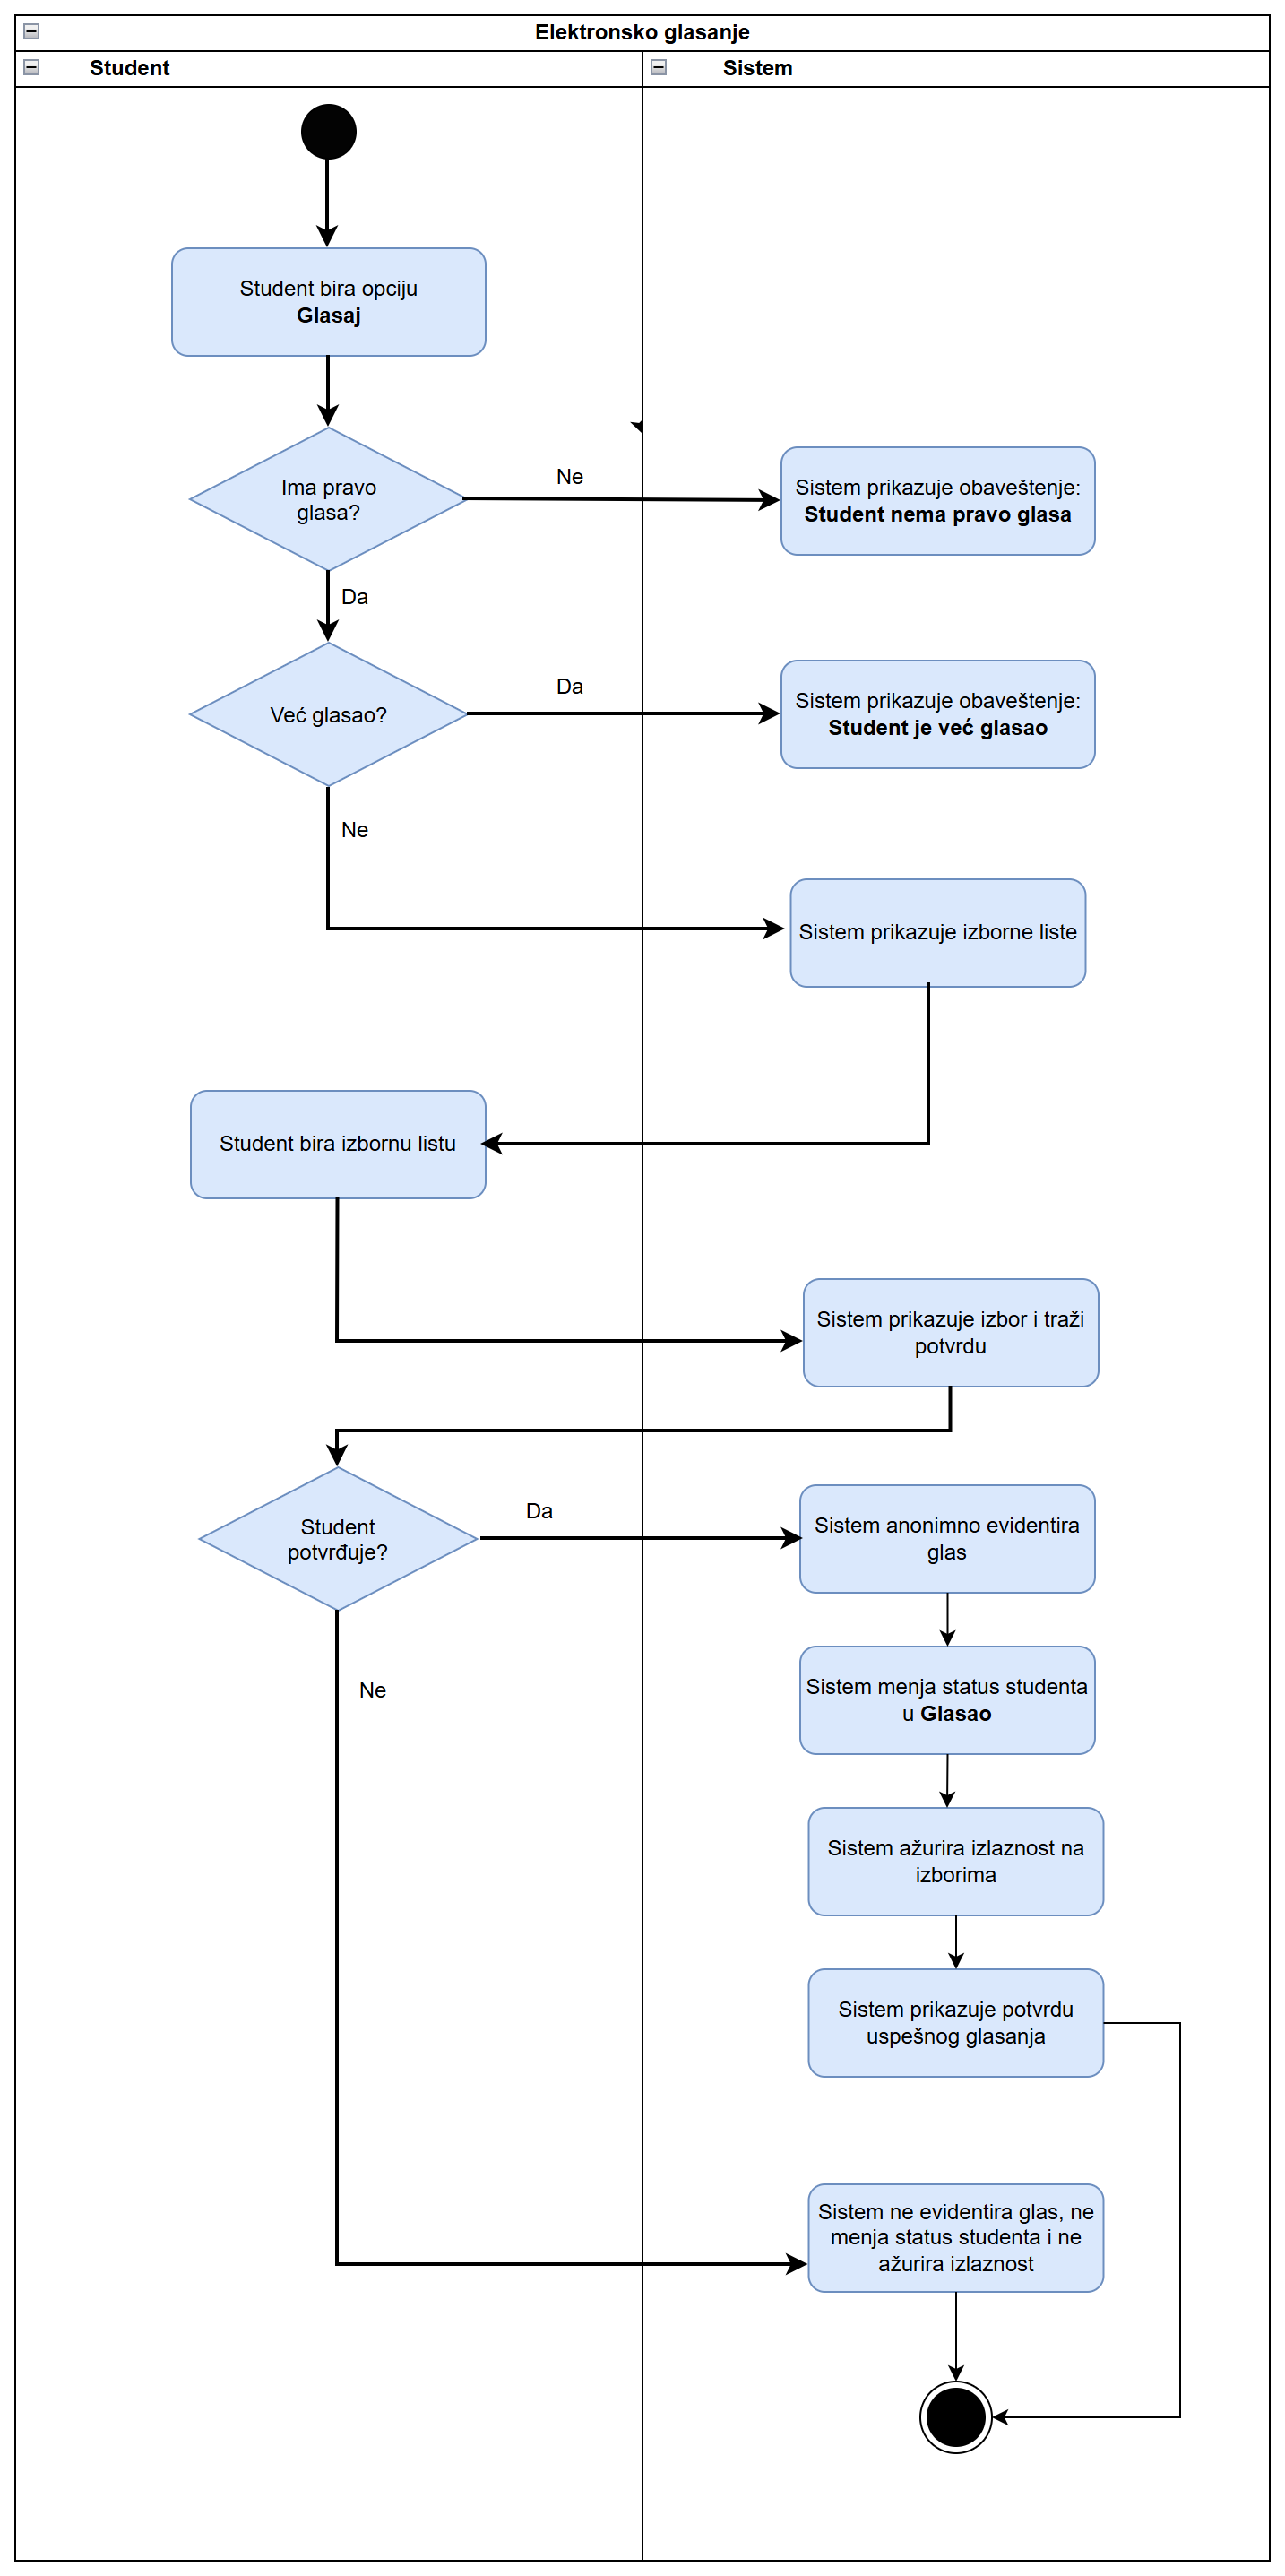
\includegraphics[height=0.8\textheight]{elektronsko_glasanje.png}
    \caption{Dijagram aktivnosti: Elektronsko glasanje}
    \label{fig:elektronsko_glasanje}
\end{figure}

\begin{figure}[H]
    \centering
    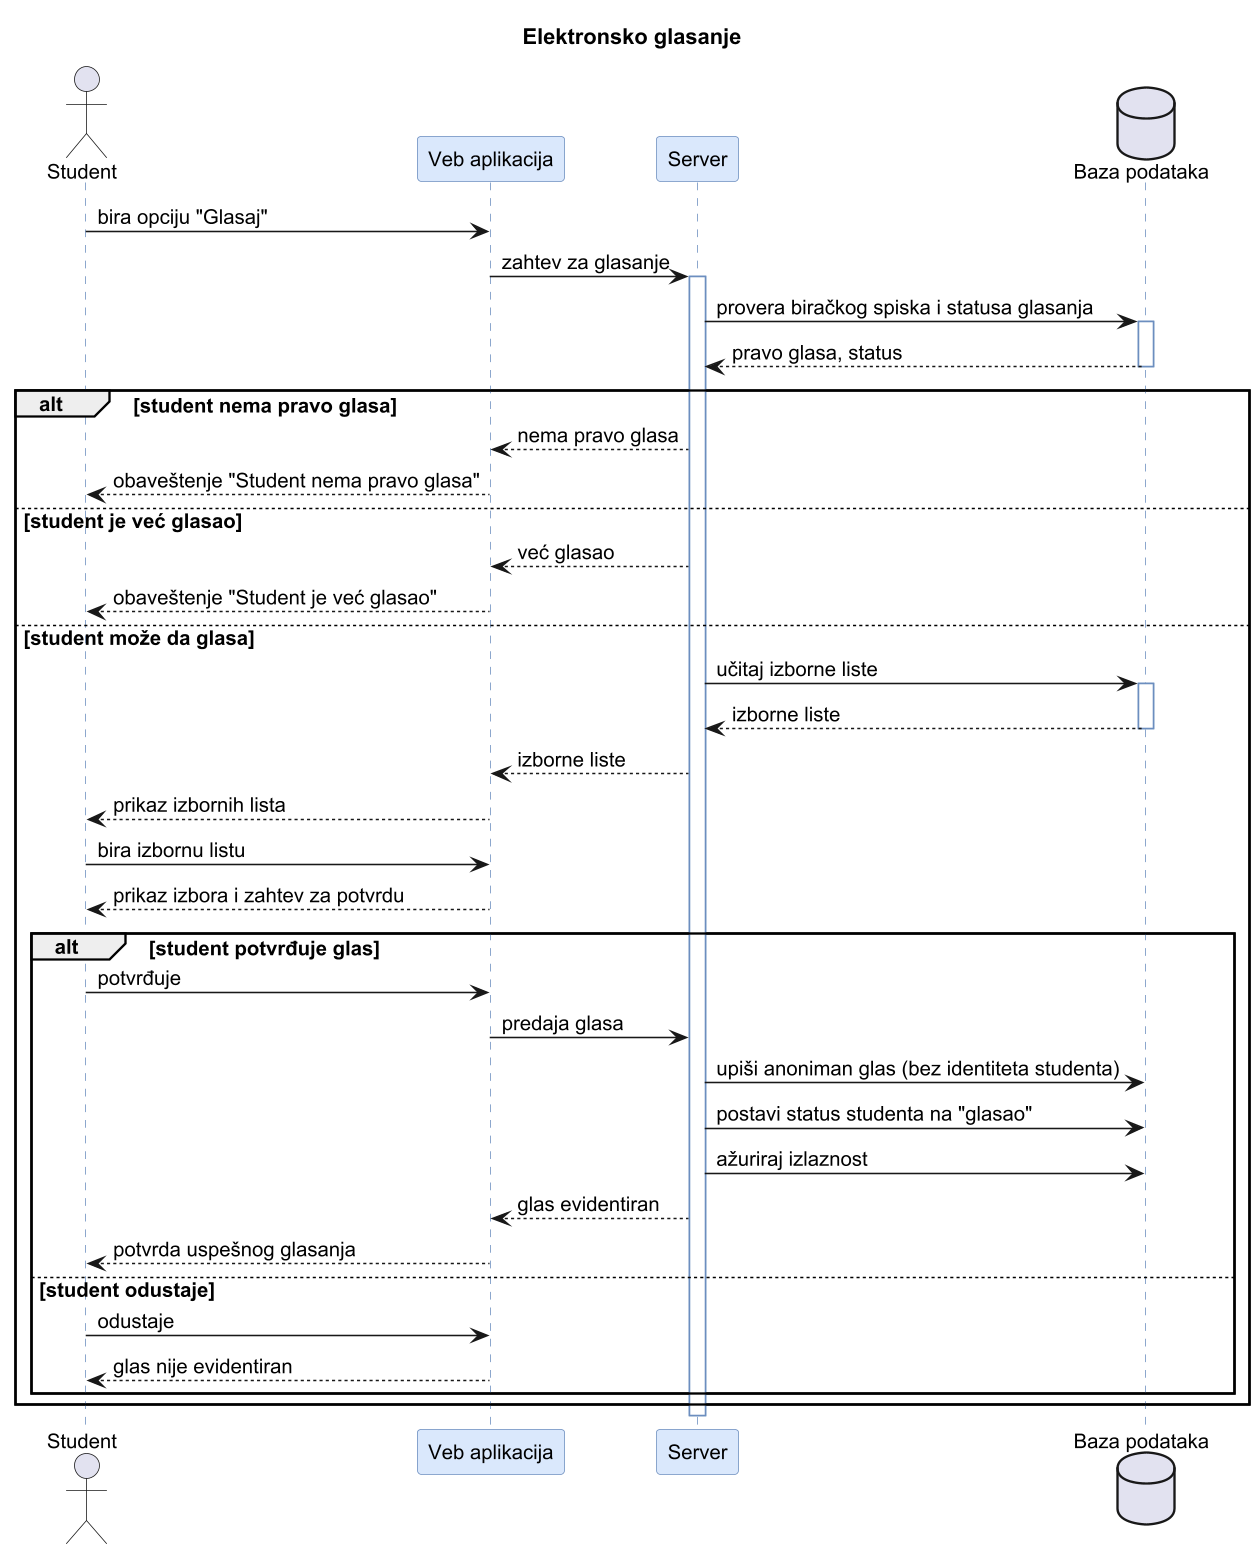
\includegraphics[width=\textwidth,height=0.8\textheight,keepaspectratio]{sekvenca_elektronsko_glasanje.png}
    \caption{Dijagram sekvence: Elektronsko glasanje}
    \label{fig:sekvenca_elektronsko_glasanje}
\end{figure}

\newpage
